\documentclass{acm_proc_article-sp}
\usepackage{graphicx}
\usepackage{mathtools}
\usepackage{color}
\usepackage[utf8x]{inputenc}
\usepackage{parskip}

\setlength{\parindent}{0pt}
\setlength{\parskip}{\baselineskip}

\begin{document}

\title{Access Control Policy Verification and Repairing in Alloy}

\numberofauthors{1}

\author{
\alignauthor Alexandr Murashkin, Ming Matthew Ma \\
       \affaddr{The David R. Cheriton School of Computer Science}\\
       \affaddr{University of Waterloo}\\
       \affaddr{Waterloo, ON, Canada}\\
       \email{m22ma, amurashk@uwaterloo.ca}
}
\date{6 December 2012}
\maketitle

\begin{abstract}
Sensitive data are becoming available through the Web and other distributed protocols. This heightens the need to carefully control access to data. Control means not only preventing the leakage of data but also permitting access to necessary information. Access control requires authorization rules and constraints. To express access control policies, several languages,
such as XACML are used to specify which subjects can  access sets of resources
or services to perform specific actions. 

We develop a tool based on first order logic modeling to detect and visualize possible conflicts within sets of access control policies expressed in XACML. We first translate the model
into a relational first order logic language called Alloy, and then analyze interactions
and conflicts among access control policies using Alloy analyzer. We then proposes potential repairs to the user thorough user interface, and automatically apply the fixes specified by the user. It is proved that with our tool can automatically determine inconsistencies in user specified model, and recommend the user and apply the repair successfully. 

\end{abstract}

\category{D.2.4}{Software Engineering}{Software/Program Verification}[formal methods]
\category{H.5.2}{Information Interfaces and Presentation}{User Interfaces}[Graphical user interfaces (GUI)]

\terms{Computer Aided Verification, Access Control Policy, User Interface}

\keywords{Alloy, XACML, rule set, policy set, GUI} % NOT required for Proceedings

\section{Introduction}

Important data are increasingly available on-line through the Web and other distributed protocols. This heightens the need to carefully control access to data. Access control means not only preventing the leakage of data but also permitting access to necessary information. The key goal is that the right person can access right resource on the right time.

\subsection{Motivation}

Due to growing variety of access methods, central databases must now provide data in a
large number of different contexts, each governed by specific access-control policies. Selective access control is an important mechanism in distributed system security. It can be used in order to allow a user to access only certain information, for certain purposes, at certain times, or when he or she plays a certain role. Access control is enforced by mechanisms that need to be programmed by means of policies. An organization may have many such policies, which may have been established at different times, by different people, perhaps without a clear view of all the consequences. Inconsistencies can then exist in such sets of policies. 

While policy mechanisms may be able to solve inconsistencies at a higher level, users and administrators still need to be aware of them, because they may lead to unintended system behavior. For example, a policy may be added to prevent a certain access, however in fact the access is still allowed because of another policy of higher priority, or the new policy may prevent access of someone who should remain authorized. We will show in this paper that such inconsistencies can be detected and fixed by using our tools.

\subsection{Background}


\textbf{\emph{XACML for Access Control}}\\
XACML is an OASIS standard that defines an architecture, policies and messages within an access control system. XACML generally center around attributes; attributes describe subjects, actions, and resources. For example, faculty is a value for the attribute role, which describes the subject. The names of attributes, such as role are called attribute ID, while the values bound
to them are called attribute values  (such as Faculty). The fragment of an XACML policy designating Faculty as a role is shown below:\\

\begin{verbatim}
<SubjectMatch MatchId=''...:string-equal''>
  <AttributeValue DataType=''...string''>
     Faculty</AttributeValue>
   <SubjectAttributeDesignator 
      AttributeId=''role''
      DataType=''...string''
   </SubjectAttributeDesignator>
</SubjectMatch>
\end{verbatim}

A rule in XACML specifies which decision to take as a function of the attributes. The XACML takes in a request, names and values of a set of attributes, and makes an access-control decision on it based on the specified rules. A decision can be permit, deny, or not-applicable which indicates that the requests is not handled. 

The access control policies are stored as XML files, they are structured into rules, policies and policy sets. Several rules are grouped into policies and policies are grouped into
policy sets. Rules, policies and policy sets define a target which indicates their domain of applicability. A target specifies a set of attributes and their values that should match those
given by a request. For example, if there are two policies, the first one is applied when the subject is a student, the resource is the marks file and the action is printing, and the second policy is applied
when the subject is a professor, the resource is the marks file and the action is modification. If a request from a student to print the marks file comes to the policy enforcement point, the policy decision point will only select the first policy to make a decision.

\textbf{\emph{Alloy}}\\
Alloy is a modeling language based on relational first order logic. An Alloy model is a collection of constraints that describes a set of structure. Alloy's tool, the Alloy Analyzer, is a solver that takes the constraints of a model and finds structures that satisfy them. It can be used both to explore the model by generating sample structures, and to check properties of the model by generating counterexamples. 

To model structures, Alloy uses the concepts of signature and relation. A signature is a type in Alloy. It can be considered equivalent to a class in the object oriented paradigm since a signature can be instantiated. For example, we can define a abstract general signature Element like this:
 
 \begin{verbatim}
abstract sig Element {
         attributes : Attribute -> Value}
         {attributes in values}
sig Subject, Resource, Action extends Element{}
\end{verbatim}

A relation is a structure that relates signatures and their instances. Functions are special binary relations; they map each instance from the left signature to only one instance from the right signature (the function effect maps each rule to only one effect). Constraints are represented in Alloy by facts. A fact is a logical formula that always holds. Alloy uses first order logic in an ASCII format. We can also specify predicates that could be evaluated to return true or false and functions that could return signature instances. Alloy is able to automatically instantiate and evaluate predicates.

\subsection{Related work}

Regarding access control policy verification, there are several various related approaches.
\cite{Hughes:2008:AVA:1459278.1459282} proposes encoding XACML access control policies  ordering relations and then translation of them into SAT solver for verification. \cite{4258517} describes inconsistency checking in role-based access control policies (RBAC).  \cite{Fisler:2005:VCA:1062455.1062502} proposes Margrave - a great tool for access control policies (XACML and other formats) verification and change-impact analysis. \cite{Jackson:2000:AFR:357474.355063} proposes Alloy Analyzer as first-order logic verification tool (there is a corresponding book \cite{jackson:alloy}).

For Access control policy verification in Alloy: 
1) http://www.cs.ucsb.edu/~bultan/publications/tech-report04.pdf
2 - WE USE IT!! ) http://w3.uqo.ca/notere05/documents/logrippo.pdf, need a citation.

Regarding repairing XACML access control policies, it does not seem to be a lot of prior related work. Rather than that, \cite{Zhang:2004:SVA:1029133.1029141} offers access control policies verification in the language called RW and then synthesize verified specifications in XACML. \cite{Bravo:2007:RIX:1783534.1783545} considers another type of access control policies - XML write access control policies - offers repairs in case of that some actions can be simulated by multiple another actions. 

Regarding model repairing in general, \cite{Xiong:2009:SAM:1595696.1595757} proposed .... for i don't know what, need to read :) . \cite{Reder:2012:CRT:2351676.2351707} proposes repair trees for inconsistency solving in design models.

The proposed technique of repairing inconsistencies - sketching - was described in the thesis http://people.csail.mit.edu/asolar/papers/thesis.pdf .

Need to look at this - probably needed - http://people.csail.mit.edu/eskang/talks/mit-security-seminar-nov2012.pdf .

The specification of XACML:
%http://docs.oasis-open.org/xacml/2.0/access_control-xacml-2.0-core-spec-os.pdf

\section{Problem Statement}

Although XACML has already achieved a considerable degree of industrial acceptance, by itself, it is impossible to determine inconsistencies and apply the fixes to repair the access control model. Inconsistencies exists as an organization may have many such policies, which may have been established at different times, by different people, perhaps without a clear view of all the consequences. 

Determining inconsistencies require verifications and finding counter examples. This process is time consuming depending on the choice of verification and modeling language. Once inconsistencies are found, the user has to apply fixes but there is no guarantee that the fixes can indeed repair the model without introducing new inconsistencies. Thus, the entire model construction process, model verification process/ finding inconsistencies and repairing process can be overwhelming.

In this paper, we propose a tool that we developed that can automatically determine the inconsistencies, recommend the repair to the users and apply fixes to the access control model.

\subsection{Paper structure}
The Design overview section brief overview of our mission and solution to the problem stated; we will introduces the main components of our tool and the implementation approach at different stage. We will then present the implementation details in Implementation section where we articulate our design approach and implementations. Evaluation section contains our experiment results and analysis for the results. In future work section, we discuss about our tool limitations and bring up possible future improvement; expert's comments are also included as a future references. Conclusion section summarizes completed work and the results.

\section{Implementation}

\subsection{Overview}

mnnnnnn  

\subsection{Pareto Front Table}

\begin{figure}[h]
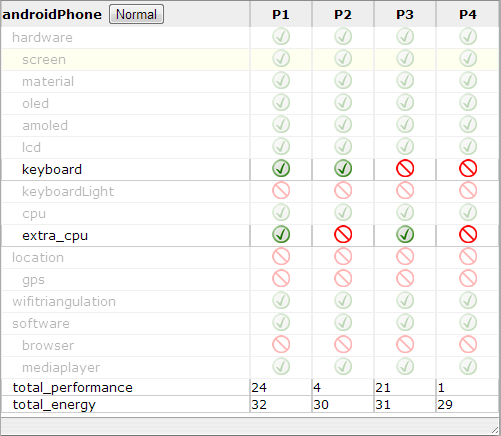
\includegraphics[width=0.5\textwidth]{table.png}
\caption{Pareto Front Table. Distinct features are highlighted}    
  \label{fig:table}
\end{figure}

Pareto Front Table (Fig.\ref{fig:table}) is a straight-forward way to represent the whole set of product configurations. Row headers represent features and total quality attributes, the hierarchical structure is preserved. Column headers represent product configurations and denoted as $P1, P2, ... PN$, $N$ - the number of generated configurations. Cells at the intersection of column $C$ and row $R$ are defined in the following way:
\begin{itemize}
\item If $R$ is a feature, and product $C$ has the feature, then the cell contains "yes" (a green tick), otherwise "no" (a red crossed circle).
\item If $R$ is a quality attribute, then the cell contains the numeric value of the quality attribute.
\end{itemize}


\section{Evaluation Result}

\subsection{Form and purpose}

The aim of the user evaluation was to determine whether visualization and interaction techniques implemented in the tool are good enough for now, and what is the further direction of development. This evaluation is a pilot study, not the final one: we are planning to conduct further evaluations with our industry partners.

To evaluate our tool, we performed a controlled experiment in which the participants were asked to perform a predefined set of tasks using the tool and answer provided questions. Occasionally, we also asked additional questions as appropriate in the given context.

The experiment included 11 tasks split into 3 groups based on the difficulty level followed by a final questionnaire (Appendix \ref{A}). Difficulty levels made the main part of the experiment well-structured and reduced learning effect. The final questionnaire was used to get an informal feedback upon the tasks completion. Three subjects - two full-time graduate students and one postdoctoral fellow of Generative Software Development Lab, University of Waterloo. All three subjects have background in product lines development and two subjects have expertise in multi-objective optimization, so no background questionnaire was used to determine their background. Prior to the experiment, we gave a short presentation of tool features to the participants, intended ways of using the tool, and completion of some sample tasks.

\subsection{Results}
asda


\section{Future work}

Although our tool demonstrate potential value in automated access control model repair, while significantly reducing user's manual work, we see future improvements in our tool. During implementation and testing stages, we noticed the following limitations in our tool:

\begin{enumerate}
\item Verification is bounded
\item Can verify one property in a time until first counterexample is found
\item Subset of XACML is covered
\item Repair procedure depends on the property and requires pre-defined prospective repair ways
\end{enumerate}

The first two points are pretty clear; our verification is bounded. Although this enables us to use Alloy as it is for bounded model checking, we would have significant dependability to Alloy. In this case, software upgrade in Alloy would cause potential mul-functioning of our tool which needs to be addressed in the future. In this project, we mainly interfaced the communication with Alloy API therefore, in the future, we need to communicate with Alloy back-end to prevent this problem.

Although we strive to make our tool scalable, the automated Alloy model generation from a user specified table brings limitations in the structure of the model we generate. Although this access control model works well for our present study, it only represents a subset of XACML. In the future, we would like to explore different ways to increase the flexibility of our model. One potential way is to incorporate sketching techniques and having multiple rule tables so that the user can choose the structure of the model our tool generates.

State explosion is not addressed in a smart way due to time constraints. We limit the depth of the potential solution to two. This obviously will become a problem when the examples are large or more complicated. We would like to study more on ways, such as graph theory and multi-object optimization to deal better with this common problem in verification and repair.

One important future improvements is on the repair recommendation. Currently, we only proposes repair based on rule effect and override effect. We derived these to approach from observation and testing. We will explore other factors such as relation, and derivation in the future to enhance our repair framework.

\section{Conclusion}

\subsection{Summary}

sfsfdfd

\subsection{Implications}

\begin{itemize}
\item Four-dimensional Pareto front visualizations can be effectively implemented using bubble charts.

\end{itemize}

\bibliography{sigproc-sp}{}
\bibliographystyle{plain}

\appendix
\section{User experiment tasks and questionnaire} \label{A}

\underline{ \textbf{I. Introductory presentation}}

\underline{ \textbf{II. Tasks}}

Tasks are split into 3 categories: \textbf{Overview}, \textbf{Graph} and \textbf{Case Studies}. All tasks are to be performed using the think-aloud protocol, that is, the participants should verbally describe what and why they are doing. All tasks are based on the file \textit{AndroidSampleMoo\_4.cfr}.

\textbf{1. Overview:}

\textbf{T1.} Upload a model file \textit{AndroidSampleMoo\_4.cfr}.\\
\textbf{T2}. Tell what features and quality attributes are specified in the Android phone model.\\
\textbf{T3}. Tell what objectives are presented in the Android phone model.\\
\textbf{T4}. Tell how many Android phone configurations are generated.\\

\textbf{2. Graph:}

\textbf{T5}. Identify 4 phones with the highest total performance (Just say: “P29, P30, P12, P4”, for instance). What is their total mass?\\
\textbf{T6}. Identify a phone with the lowest energy consumption. What is its total performance?\\
\textbf{T7}. Identify the phones with very low total mass.\\
\textbf{T8}. How many phones have perfect (highest) total security? What features contribute to total security?\\

\textbf{3. Cases studies:}

\textbf{T9.} Your boss says that among all the sets of phones you need to issue only one. He says that he needs to choose one among the phones with the best total performance. He is OK with any high energy consumption, since new Android battery is very good. He says he does not need a perfect total security, but it should be more than 0. So he is OK to sacrifice total security to get more total performance.\\
\textit{Your actions:}\\
1) Which product(s) will you choose and why?\\

\textbf{T10.} Your boss says that it is interesting that bubbles representing P5, P8, P2, and P22 are located close to each other. And he wants to know why this happened. Because, maybe, the phones are equivalent in some sense and we can consider them separately as an equivalence class.\\
\textit{Your actions:}\\
1) What do the products have in common and what are the differences?\\
2) Why the bubbles are located close to each other?\\

\textbf{T11.} Your boss needs you to analyze the total performance and total mass of all prospective phones that have USB and WiFi features. He knows that P5, P8, P2, P22 and P18 have USB and WiFi. But he wants to consider all the phones that have USB and WiFi features.\\
\textit{Your actions:}\\
1) Make the set to be a complete equivalence class by adding other relevant products to it.\\
2) Among the selected products within the equivalence class, what is the:\\
	Minimal,\\
	Mean,\\
	Maximal\\
total performance? Are the phones differ in total mass significantly or not?\\
3) Based on the question above, is it reasonable for the boss sacrifice total mass to gain more total performance?\\

\underline{ \textbf{Questionnaire}}\\

\textbf{Q1.} Do you find the idea of representing the products in a four-dimensional space using bubble chart useful? Any comments on that? Are there limitations? Does the representation of the four dimensions make it easy to find “better” products?\\
\textbf{Q2.} What do you think about the notion of the complete equivalence class? What is it and how it can be used? Describe it in your own words.\\
\textbf{Q3.} I noticed that I can group products together based on their features, so each cluster will be denoted by an equivalence class. Let’s call it “clustering by features”. Do you think it is a good idea or not?\\



\balancecolumns
\end{document}
